\newpage
\setcounter{subsection}{0}
\section{ANÁLISIS DEL PROBLEMA}

\subsection{Requerimientos}

El sistema se especifica mediante veinte requerimientos funcionales (RF) y veinte requerimientos no funcionales (RNF), organizados en cinco módulos: M1 gestión de eventos y tickets, M2 emisión NFT, M3 mercado secundario, M4 configuración y políticas, M5 usuarios y autenticación. La especificación detallada con criterios de aceptación y trazabilidad a casos de uso se entrega como anexo (SRS). Las Tablas~\ref{tab:rf} y~\ref{tab:rnf} resumen el conjunto completo.

\begin{table}[H]
\centering
\scriptsize
\caption{Requerimientos funcionales del sistema (resumen).}
\label{tab:rf}
\begin{tabular}{p{1.2cm}p{11.2cm}p{1.6cm}}
\toprule
\textbf{Id.} & \textbf{Descripción} & \textbf{Módulo} \\
\midrule
RF-01 & Comprar boletos para un evento mediante interfaz clara. & M1, M5 \\
RF-02 & Validar que la compra sea autorizada (reglas, permisos, control de usuario). & M1, M4, M5 \\
RF-03 & Generar identificador único para cada boleto, vinculable al NFT. & M1, M2 \\
RF-04 & Permitir compra con flujo sencillo. & M1, M5 \\
RF-05 & Autenticar al usuario antes de comprar. & M5 \\
RF-06 & Registrar propietario inicial y final del boleto (trazabilidad). & M1, M2, M3, M5 \\
RF-07 & Listar boleto para reventa. & M3, M4, M5 \\
RF-08 & Verificar que el usuario sea dueño antes de revender. & M2, M3, M5 \\
RF-09 & Ejecutar compra en reventa de forma atómica. & M2, M3, M4, M5 \\
RF-10 & Evitar que el boleto se venda más de una vez. & M1, M2, M3 \\
RF-11 & Ejecutar proceso de \textit{burn} del boleto vendido. & M2, M3 \\
RF-12 & Generar nuevo token para nuevo propietario. & M2, M3, M5 \\
RF-13 & Mantener historial de transferencias. & M1, M2, M3, M5 \\
RF-14 & Consultar estado de boletos adquiridos. & M1, M2, M5 \\
RF-15 & Verificación rápida del boleto. & M1, M2 \\
RF-16 & Solo el propietario puede modificar el precio de reventa. & M3, M4, M5 \\
RF-17 & Integrarse con contratos inteligentes Soroban. & M2, M3, M4 \\
RF-18 & Modificar precio del boleto listado para reventa. & M3, M4, M5 \\
RF-19 & Consultar disponibilidad de boletos. & M1 \\
RF-20 & Registrar cada transacción realizada. & M1, M2, M3, M5 \\
\bottomrule
\end{tabular}
\end{table}

Los RNF cubren desempeño, seguridad, usabilidad, disponibilidad, mantenibilidad e integración.

\begin{table}[H]
\centering
\scriptsize
\caption{Requerimientos no funcionales del sistema (resumen).}
\label{tab:rnf}
\begin{tabular}{p{1.2cm}p{12.8cm}}
\toprule
\textbf{Id.} & \textbf{Descripción} \\
\midrule
RNF-01 & Procesar la compra de boletos en menos de 5 segundos. \\
RNF-02 & Soportar al menos 100 usuarios concurrentes. \\
RNF-03 & Tener disponibilidad mínima del 99{,}5\,\% mensual. \\
RNF-04 & Bloquear transacciones tras 3 intentos fallidos consecutivos. \\
RNF-05 & Cifrar comunicaciones mediante TLS 1.2 o superior. \\
RNF-06 & Soportar al menos 2\,400 transacciones diarias. \\
RNF-07 & Completar el proceso de compra en máximo 5 pasos. \\
RNF-08 & Permitir aprendizaje del usuario en menos de 15 minutos. \\
RNF-09 & Mantener una tasa de fallos menor al 0{,}5\,\%. \\
RNF-10 & Garantizar atomicidad en el 100\,\% de las transacciones. \\
RNF-11 & Tener cobertura de pruebas mínima del 70\,\%. \\
RNF-12 & Ser compatible con navegadores web modernos. \\
RNF-13 & Integrarse con contratos Soroban mediante API REST. \\
RNF-14 & Almacenar \textit{logs} por mínimo 12 meses. \\
RNF-15 & Cerrar sesión tras 30 minutos de inactividad. \\
RNF-16 & No superar 5 horas de inactividad mensual. \\
RNF-17 & Verificar boletos en menos de 5 segundos. \\
RNF-18 & Soportar varios eventos simultáneos. \\
RNF-19 & Recuperarse de fallos en menos de 20 minutos. \\
RNF-20 & Conservar historial de boletos por mínimo 5 años. \\
\bottomrule
\end{tabular}
\end{table}

\subsection{Restricciones}

Las restricciones del prototipo se agrupan en cuatro categorías:

\begin{itemize}\setlength{\itemsep}{2pt}
    \item \textbf{De alcance.} El sistema se limita al mercado secundario de entradas para eventos de entretenimiento. Quedan fuera la integración con pasarelas de pago fiat reales, los procesos KYC, el despliegue en \textit{mainnet} y el acoplamiento con plataformas comerciales de \textit{ticketing}.
    \item \textbf{Técnicas.} El despliegue se realiza sobre la red de prueba (\textit{testnet}) de Stellar. La compra del comprador final se firma exclusivamente desde la extensión Freighter en el navegador. Las operaciones clásicas (\texttt{change\_trust}, \texttt{payment}) se enrutan por Horizon; las invocaciones de contrato, por Soroban RPC. El indexador no se ejecuta en entornos \textit{serverless} dado que requiere proceso de fondo persistente.
    \item \textbf{Normativas.} La Ley 1493 de 2011 se incluye como referencia académica para la fiscalización digital de espectáculos públicos en Colombia.
    \item \textbf{Operativas.} La política de comisiones del prototipo se fija en 5\,\% organizador y 3\,\% plataforma; estos parámetros son configurables por contrato pero no se modifican durante la evaluación. La ventana de retención del método \texttt{getEvents} del RPC público obliga al indexador a poll-ear cada 5 segundos.
\end{itemize}

\subsection{Especificación Funcional}

El sistema involucra cuatro actores principales, alineados con los casos de uso del SDD. Cada rol queda acotado y, cuando interviene on-chain, queda verificado por el contrato mediante \texttt{require\_auth()} sobre la dirección Stellar correspondiente:

\begin{itemize}\setlength{\itemsep}{2pt}
    \item \textbf{Administrador de la Plataforma.} Configura eventos en el panel administrativo y dispara el despliegue de contratos de evento mediante el \texttt{factory\_contract}.
    \item \textbf{Organizador del evento (ticketera B2B).} Única dirección autorizada para invocar \texttt{crear\_boleto}, registrar verificadores e invalidar boletos en un contrato de evento. Es receptor de las comisiones de organizador.
    \item \textbf{Usuario.} Comprador y vendedor del mercado primario y secundario. El propietario actual firma \texttt{listar\_boleto} y \texttt{cancelar\_venta}; el comprador firma \texttt{comprar\_boleto} desde Freighter.
    \item \textbf{Personal del Evento (verificador en puerta).} Rol \texttt{STAFF} o \texttt{ADMIN} registrado por el organizador. Ejecuta la redención en puerta a través del endpoint \texttt{POST /api/admin/scan}, con respaldo on-chain mediante \texttt{redimir\_boleto}.
\end{itemize}

El diagrama de casos de uso (Figura~\ref{fig:cu}) sintetiza la interacción de los cuatro actores con las funcionalidades principales del sistema, agrupadas por módulo. La especificación detallada de cada caso de uso (CU-01 Crear evento y desplegar contrato, CU-02 Compra primaria, CU-03 Listar para reventa, CU-04 Compra en reventa atómica, CU-05 Verificar en puerta, CU-06 Invalidar boleto) se documenta en el anexo SDD.

\begin{figure}[H]
\centering
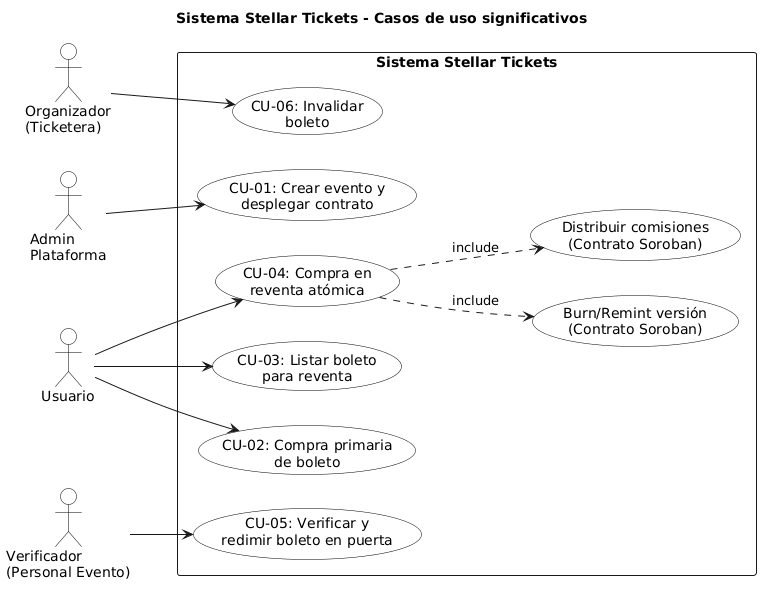
\includegraphics[width=0.95\textwidth]{Imagenes/CasosDeUso_SAD.png}
\caption{Diagrama de casos de uso del sistema (4 actores, 6 casos de uso principales).}
\label{fig:cu}
\end{figure}

El ciclo de vida funcional del boleto comprende seis fases observables on-chain: \textit{creación} por parte del organizador; \textit{listado} en mercado secundario; \textit{compra} (primaria o reventa); \textit{transferencia de propiedad} mediante \textit{burn/remint}; \textit{redención} por un verificador autorizado; y \textit{cancelación administrativa} por el organizador en casos excepcionales. Las consultas de solo lectura cubren la verificación de propiedad, la versión vigente, el conjunto de boletos en reventa y el historial completo del evento.

La especificación detallada de casos de uso, los criterios de aceptación por operación y la trazabilidad entre RF, operaciones del contrato y pruebas unitarias se documentan en el anexo SRS.
